Soit la fonction $f$ définie et dérivable sur $[0\,;\,10]$ par :\quad $f(x)=-x^{3}+4{,}5\,x^{2}-6x+2$.
	
	\begin{enumerate}
		\item Calculer l'expression de la dérivée $f'$ en fonction de $x$.
		
		\begin{color}{blue}
		On utilise la dérivation d'une somme de fonctions dérivables.
		
		$f'(x)=(-1)\times 3x^{2} + 4{,}5\times 2x - 6  = -3x^2 + 9x - 6$
		
		\end{color}
		
		
		\item Vérifier que, pour $x$ appartenant à $[0\,;\,10]$, $f'(x)=(3x-6)(1-x)$.

		\begin{color}{blue}
		On développe l'expression :
		
		\(
		(3x-6)(1-x) = 3x\times 1 +3x\times (-x) + (-6)\times 1 (-6)\times (-x) 
		\)
		
		On réduit les produits :
		
		\(
		(3x-6)(1-x) = 3x -3x^2 - 6 + 6x 
		\)
		
		
		On réduit les sommes :

		\(
		(3x-6)(1-x) = -3x^2 + 9x - 6  
		\)
		
				
		\end{color}
		
		\item Étudier le signe de $f'(x)$ pour $x$ appartenant à $[0\,;\,10]$.
		
		\begin{color}{blue}
		Pour étudier le signe de $f'(x)$, on étudie le signe de chacun des facteurs de l'expression factorisée de $f'(x)=(3x-6)(1-x)$.
		
		$3x - 6 = 0 \iff 3x = 6 \iff x = 2$
		
		$3x - 6 > 0 \iff 3x > 6 \iff x > 2$
		
		$1 - x = 0 \iff 1 = x \iff x = 1$
		
		$1 - x > 0 \iff 1 > x \iff x < 1$
		
		On forme le tableau de signes :
		
		
		\begin{center}
				\begin{tikzpicture}
					\tkzTabInit[lgt=3.5,espcl=1.4]
					{$x$/0.7,$3x-6$/0.7,$1-x$/0.7,signe de $f'(x)$/1.4}
					{$0$,$1$,$2$,$10$}
				\tkzTabLine{,-, ,+, z,+,}
				\tkzTabLine{,+, z,-,,-,}
				\tkzTabLine{,-,z,+,z,-,}
			\end{tikzpicture}
		\end{center}
		
		 
				
		\end{color}
		
		\item En déduire les variations de $f$ sur $[0\,;\,10]$.
		
		Les valeurs des éventuels maximums et minimums ne sont pas demandées.
		
		\begin{color}{blue}
		\begin{center}
				\begin{tikzpicture}
					\tkzTabInit[lgt=3.5,espcl=1.4]
					{$x$/0.7,signe de $f'(x)$/1.4,variation de $f$/2.4}
					{$0$,$1$,$2$,$10$}
				\tkzTabLine{,-,z,+,z,-,}
				\tkzTabVar{+/,-/,+/,-/}
			\end{tikzpicture}
		\end{center}
		\end{color}
		
	\end{enumerate}
